\documentclass{article}
\usepackage[margin=1in]{geometry}
\usepackage{tikz}
\usetikzlibrary{shapes.geometric, arrows, positioning}
%For tikz node diagram setup
\pagenumbering{gobble}

\definecolor{mgreen}{HTML}{689562}
\definecolor{mpurp}{HTML}{85678f}
\definecolor{mblue}{HTML}{3C406C}
\definecolor{mgray}{HTML}{6F6F6F}
\tikzset{trapezium stretches=true}
\tikzstyle{source} = [rectangle, rounded corners, minimum width= 2cm, minimum height = 1cm, text = white, text centered, fill = mgray]
\tikzstyle{input} = [trapezium, trapezium left angle=50, trapezium right angle = 130, minimum width = 1.5cm, minimum height=1cm, text centered, text=white, fill=mgreen]
\tikzstyle{routing} = [diamond, minimum width=2cm, minimum height=1cm, aspect = 2, text width = 2cm, text centered, text=white,fill = mblue]
\tikzstyle{processor} = [rectangle, minimum width = 2cm, minimum height = 1cm, text width = 3cm, text = white, fill = mpurp]
\tikzstyle{cable} = [thick, ->, >=latex]
\tikzstyle{usb} = [thick, <->, >=latex]


\begin{document}
\centering
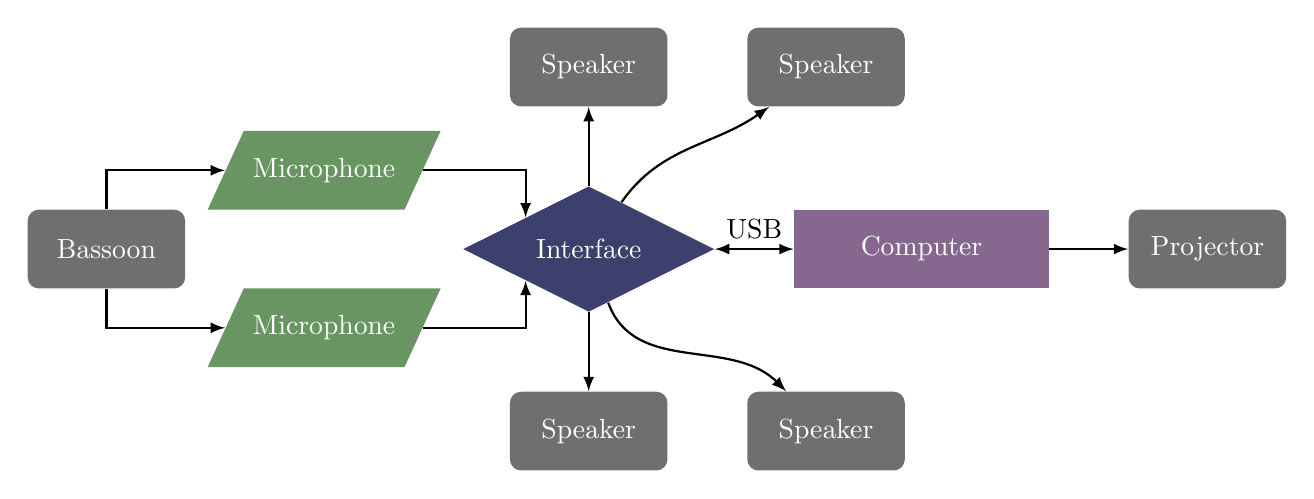
\begin{tikzpicture}[align=center,node distance = 1cm]
  \node (bsn) [source] {Bassoon};
  \node (mic1) [input, right= of bsn, yshift = 1cm, xshift=-0.5cm] {Microphone};
  \node (mic2) [input, right= of bsn, yshift = -1cm, xshift=-0.5cm] {Microphone};
  \draw [cable] (bsn) |- (mic1);
  \draw [cable] (bsn) |- (mic2);
  \node (mixer) [routing, right = of mic1, yshift = -1cm, xshift= -0.5cm] {Interface};
  \draw [cable] (mic1) -| (mixer.north west);
  \draw [cable] (mic2) -| (mixer.south west);
 \node (speaker1) [source, above = of mixer] {Speaker};
  \node (speaker2) [source, below = of mixer] {Speaker};
  \node (speaker3) [source, right= of speaker1] {Speaker};
  \node (speaker4) [source, right= of speaker2] {Speaker};
  \node (computer) [processor, text width = 3cm, right = of mixer] {Computer};
  \node (video) [source, right= of computer] {Projector};
  \draw [usb] (mixer) -- node[anchor = south] {USB} (computer);
  \draw [cable] (mixer) -- (speaker1);
  \draw [cable] (mixer) -- (speaker2);
  \draw [cable] (mixer) to[out=55, in=215] (speaker3);
  \draw [cable] (mixer) to[out=-70, in=135] (speaker4);
  \draw [cable] (computer) -- (video);
\end{tikzpicture}


\end{document}
